\cohead{\Large\textbf{Integrale - grafische Interpretation}}
\fakesubsection{Grafische Interpretation von Integralen}
Das (bestimmte) Integral von \(f(x)\) zwischen \(x=a\) und \(x=b\) mit \(a<b\) wird wie folgt aufgeschrieben:
\[\textcolor{loes}{\int_a^b f(x)\td x}\]
\begin{itemize}
	\item \(a\): \textcolor{loes}{Obere Integrationsgrenze}\\
	\item \(b\): \textcolor{loes}{Untere Integrationsgrenze}\\
	\item \(f(x)\): \textcolor{loes}{Integrand bzw. die zu integrierende Funktion}\\
	\item \(\text{d} x\): \textcolor{loes}{Variable, über die integriert wird. Bei uns immer \(x\)}\\
\end{itemize}
\begin{tcolorbox}
	\textcolor{loestc}{Im Schaubild entspricht das Integral dem \textbf{orientierten} Flächeninhalt zwischen dem Schaubild und der \(x\)-Achse im Intervall \([a;b]\). Orientiert bedeutet dabei, dass die Fläche oberhalb der \(x\)-Achse positiv gezählt wird und die Fläche unterhalb der \(x\)-Achse negativ gezählt wird. Liegt also mehr Fläche unterhalb der \(x\)-Achse als oberhalb, nimmt das Integral einen negativen Wert an.}
\end{tcolorbox}
\begin{minipage}{\textwidth}
	\begin{minipage}{.59\textwidth}\raggedright
		Betrachten wir die Funktion \(f(x)=\frac{1}{4}x^2+1\).
		\begin{align*}
			\int_0^1 \frac{1}{4}x^2+1\td x&\approx\textcolor{loes}{1,2}\\		
			\int_1^3 \frac{1}{4}x^2+1\td x&\approx\textcolor{loes}{4,2}\\
			\int_0^3 \frac{1}{4}x^2+1\td x&\approx\textcolor{loes}{5,4}
		\end{align*}		
	\end{minipage}
	\begin{minipage}{.36\textwidth}
		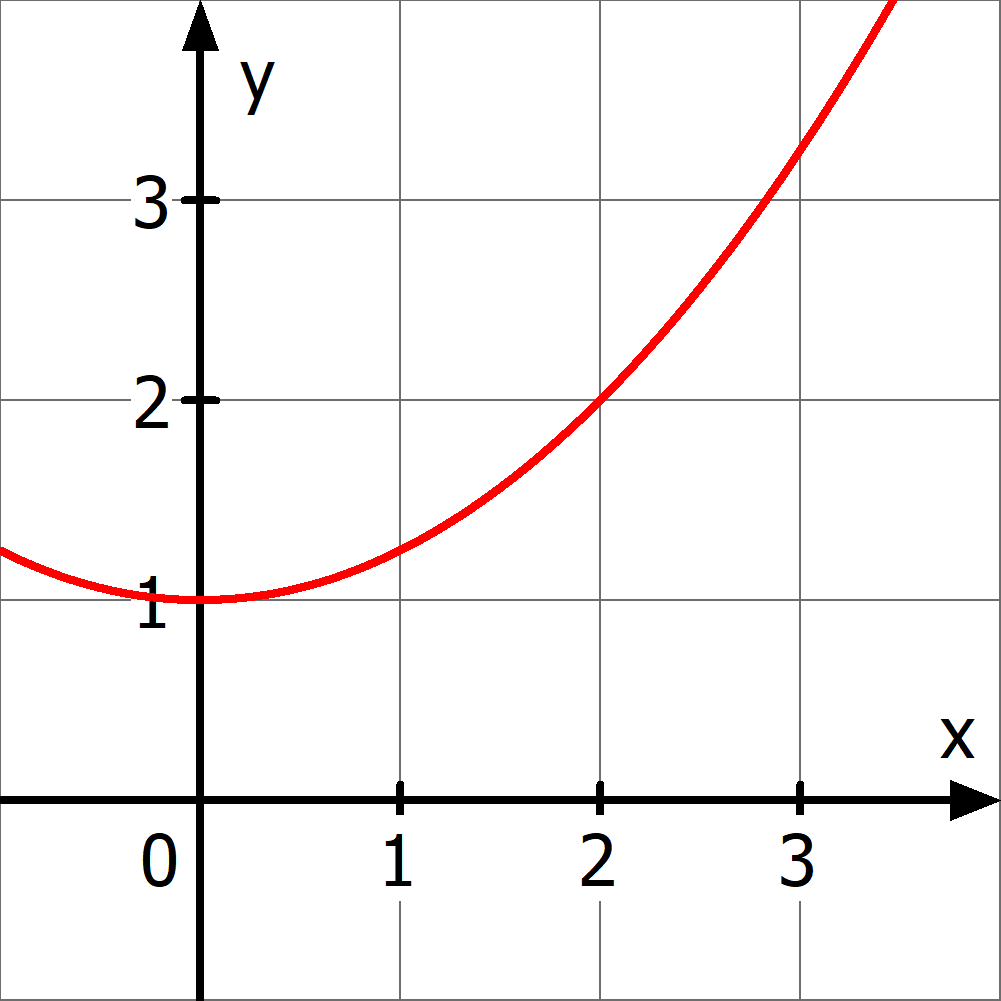
\includegraphics[width=.95\linewidth]{\integration/pics/EinViertelXQuadratPlusEins.png}
	\end{minipage}
\end{minipage}
\vspace{1cm}\\
\begin{minipage}{\textwidth}
	\begin{minipage}{.36\textwidth}
		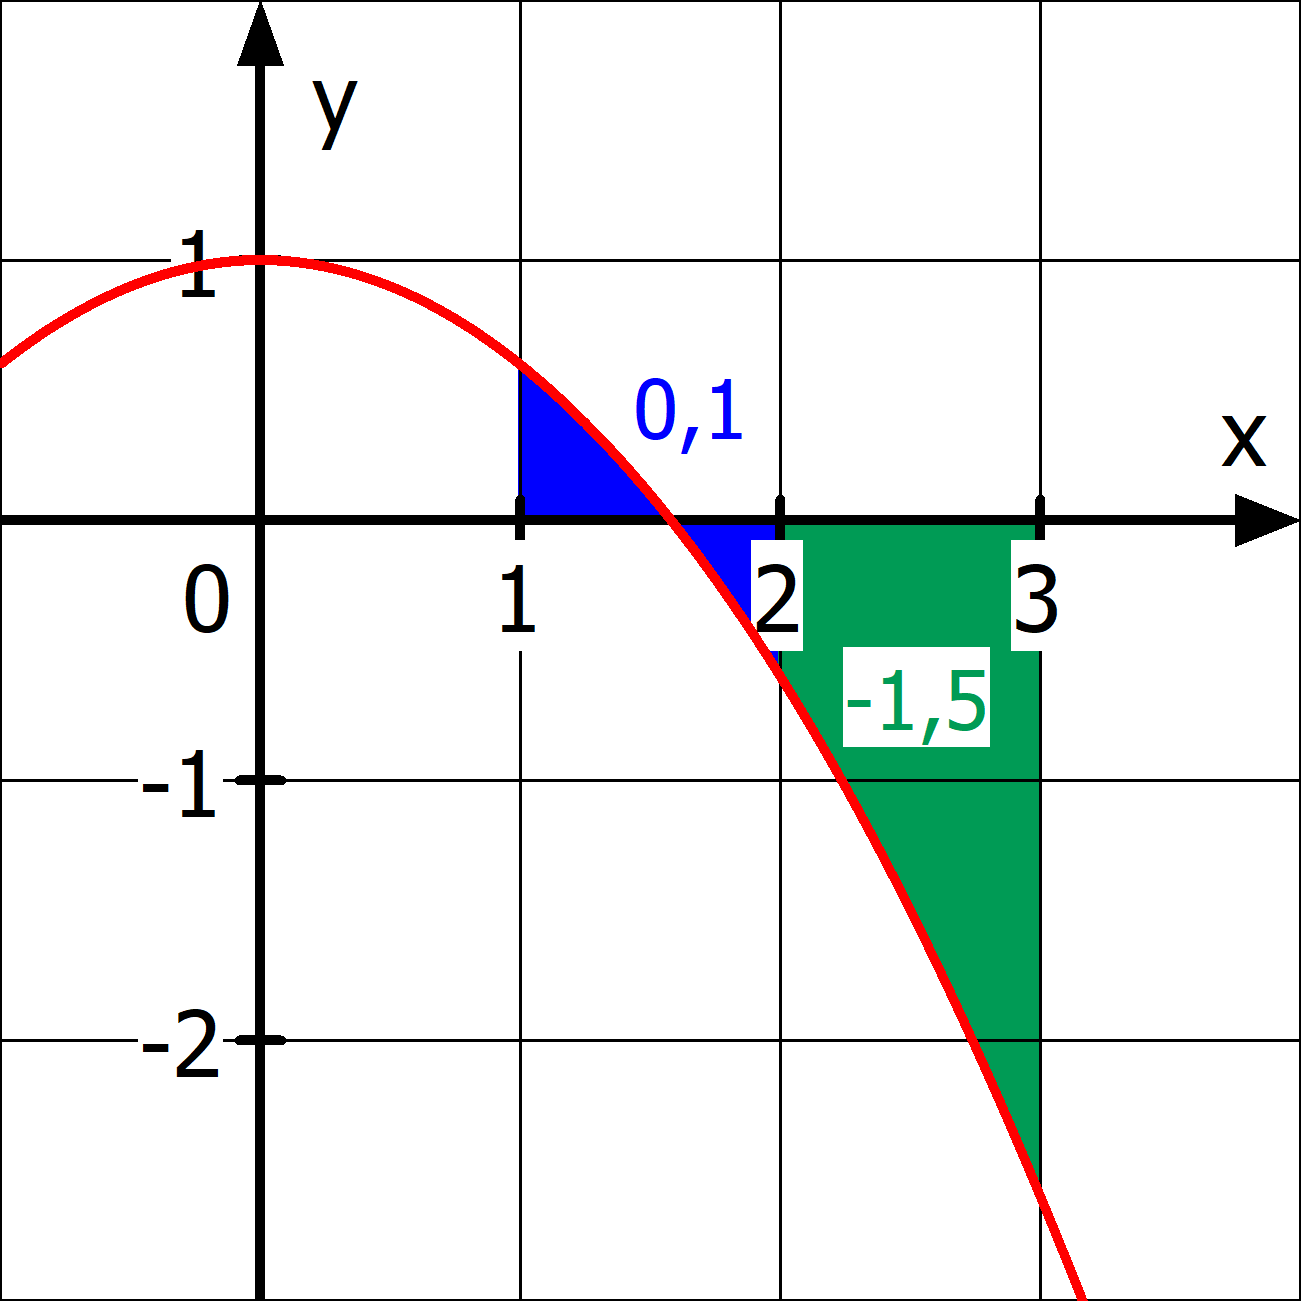
\includegraphics[width=.95\linewidth]{\integration/pics/MinusZweiFuenftelXHochZweiPlusEins.png}
	\end{minipage}
	\begin{minipage}{.59\textwidth}\raggedright
		Als zweites Beispiel betrachten wir die Funktion \(f(x)=-\frac{2}{5}x^2+1\).
		\begin{align*}
			\int_0^3 -\frac{2}{5}x^2+1\td x&\approx\textcolor{loes}{0,7}\\
			\int_1^2 -\frac{2}{5}x^2+1\td x&\approx\textcolor{loes}{0}\\
			\int_2^3 -\frac{2}{5}x^2+1\td x&\approx\textcolor{loes}{-1,4}
		\end{align*}
	\end{minipage}
\end{minipage}
\newpage
\begin{Exercise}[title={\raggedright\normalfont Schätze jeweils den Wert der Integrale zwischen der unteren Grenze \(a\) und der oberen Grenze \(b\) an Hand des Schaubilds der Funktion ab.}, label=integralGrafisch1]\\
	% GrafischA1_1.png  f(x) = -1/4*x^3+2
	% GrafischA1_2.png  f(x) = 1/3*x^2+x
	% GrafischA1_3.png  f(x) =1/10*x^3-3
	% GrafischA1_4.png  f(x) =-1/5*x^4+x^2+2
	% GrafischA1_5.png  f(x) =x^3-3*x^2+1/4*x
	% GrafischA1_6.png  f(x) =-1/3*x^2+2
	\begin{minipage}{\textwidth}
		\begin{minipage}{.33\textwidth}
			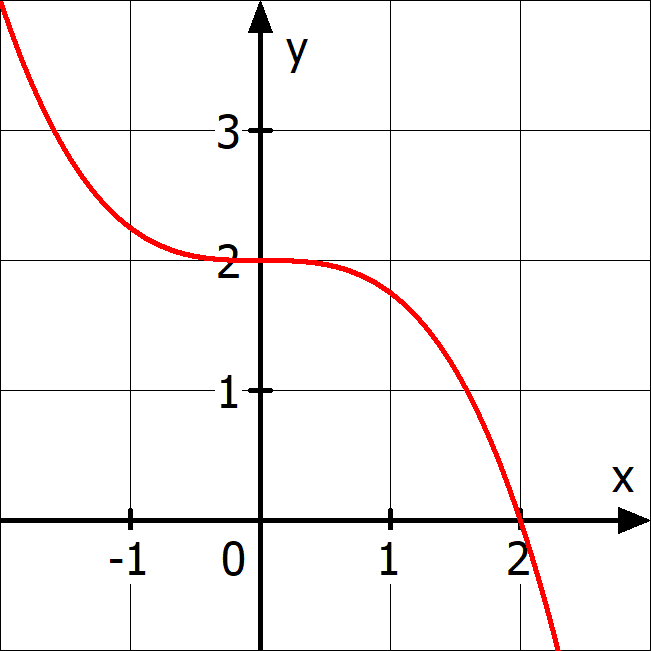
\includegraphics[width=.95\linewidth]{\integration/pics/GrafischA1_1.png}
		\end{minipage}
		\begin{minipage}{.33\textwidth}
			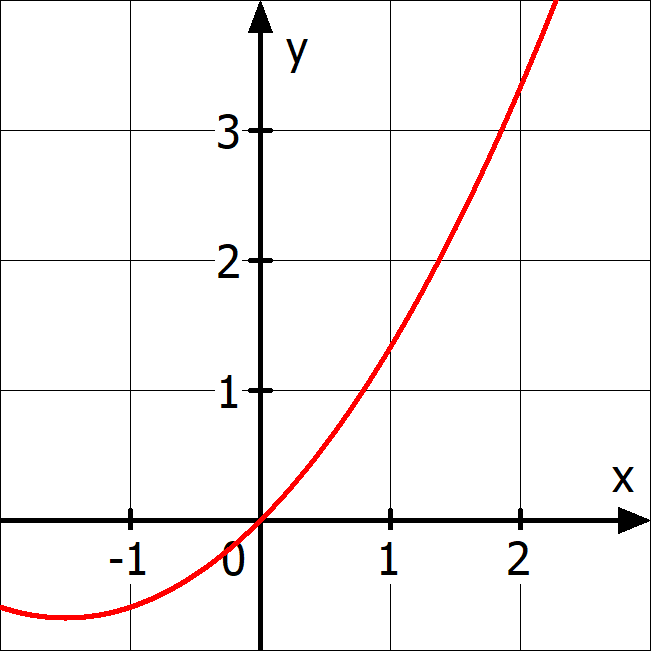
\includegraphics[width=.95\linewidth]{\integration/pics/GrafischA1_2.png}
		\end{minipage}
		\begin{minipage}{.33\textwidth}
			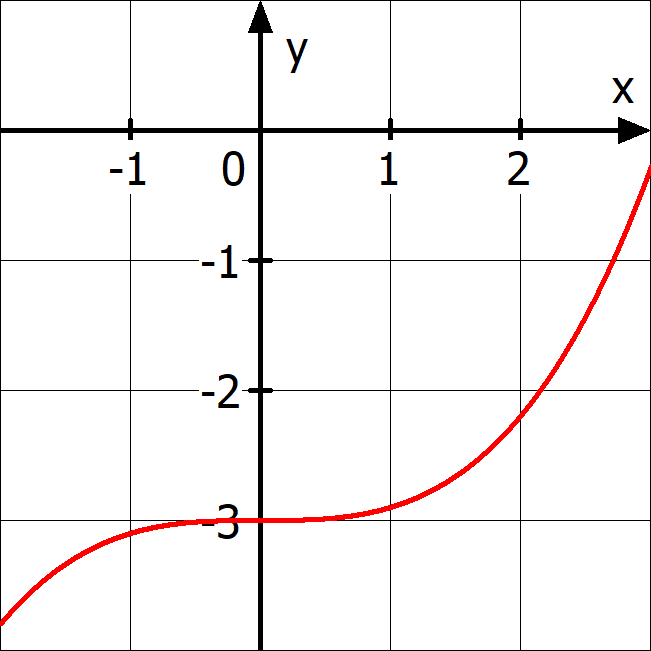
\includegraphics[width=.95\linewidth]{\integration/pics/GrafischA1_3.png}
		\end{minipage}
	\end{minipage}
	\vspace{0.3cm}\\
	\begin{minipage}{\textwidth}
		\begin{minipage}{.33\textwidth}\raggedright
			\(f(x)=-\frac{1}{4}x^3+2\)
			\begin{enumerate}[label=\alph*)]
				\setcounter{enumi}{0}
				\item \(a=-1\) und \(b=2\)
				\item \(a=-1\) und \(b=1\)
				\item \(a=0\) und \(b=2\)
			\end{enumerate}
		\end{minipage}
		\begin{minipage}{.33\textwidth}\raggedright
			\(f(x)=\frac{1}{3}x^2+x\)
			\begin{enumerate}[label=\alph*)]
				\setcounter{enumi}{3}
				\item \(a=-1\) und \(b=2\)
				\item \(a=-1\) und \(b=1\)
				\item \(a=0\) und \(b=2\)
			\end{enumerate}
		\end{minipage}
		\begin{minipage}{.33\textwidth}\raggedright
			\(f(x)=\frac{1}{10}x^3-3\)
			\begin{enumerate}[label=\alph*)]
				\setcounter{enumi}{6}
				\item \(a=-1\) und \(b=2\)
				\item \(a=-1\) und \(b=1\)
				\item \(a=0\) und \(b=2\)
			\end{enumerate}
		\end{minipage}
	\end{minipage}
	\vspace{1cm}\\
	\begin{minipage}{\textwidth}
		\begin{minipage}{.33\textwidth}
			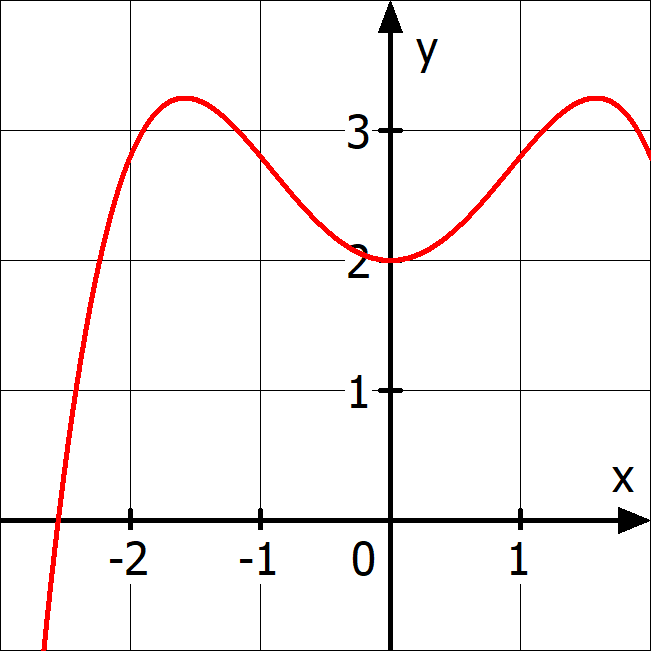
\includegraphics[width=.95\linewidth]{\integration/pics/GrafischA1_4.png}
		\end{minipage}
		\begin{minipage}{.33\textwidth}
			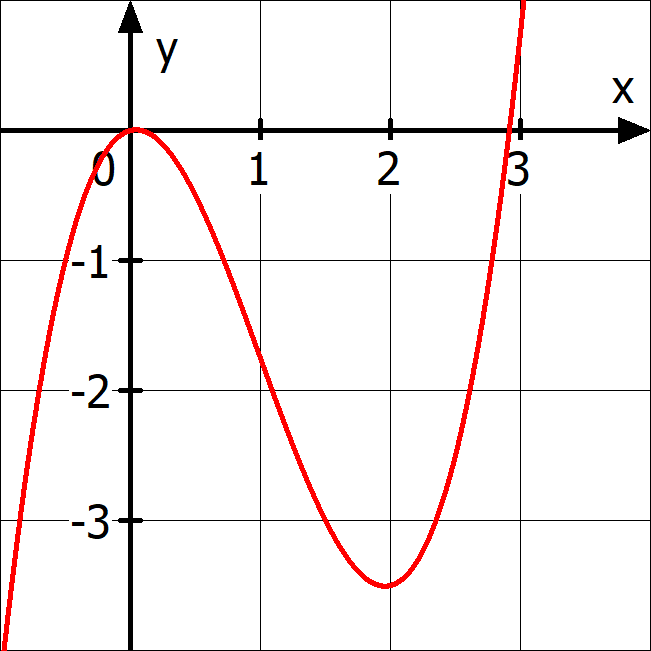
\includegraphics[width=.95\linewidth]{\integration/pics/GrafischA1_5.png}
		\end{minipage}
		\begin{minipage}{.33\textwidth}
			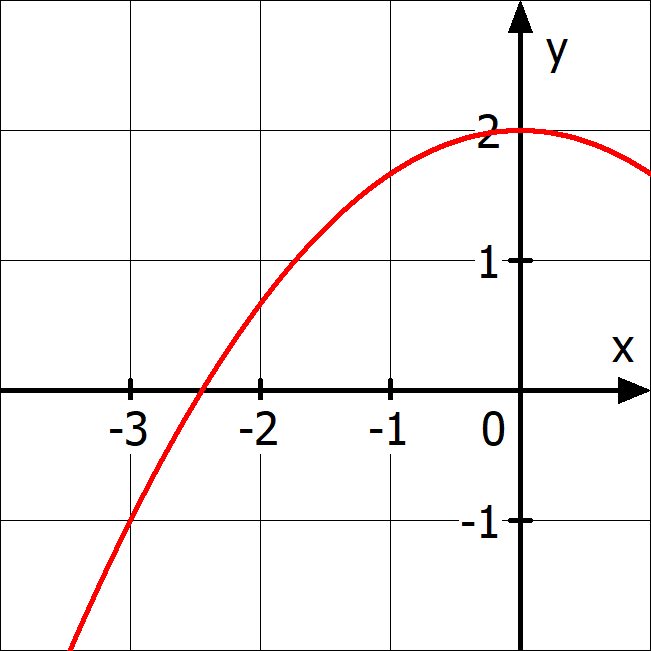
\includegraphics[width=.95\linewidth]{\integration/pics/GrafischA1_6.png}
		\end{minipage}
	\end{minipage}
	\vspace{0.3cm}\\
	\begin{minipage}{\textwidth}
		\begin{minipage}{.33\textwidth}\raggedright
			\(f(x)=-\frac{1}{5}x^4+x^2+2\)
			\begin{enumerate}[label=\alph*)]
				\setcounter{enumi}{9}
				\item \(a=-2\) und \(b=0\)
				\item \(a=-2\) und \(b=1\)
				\item \(a=-1\) und \(b=1\)
			\end{enumerate}
		\end{minipage}
		\begin{minipage}{.33\textwidth}\raggedright
			\(f(x)=x^3-3x^2+\frac{1}{4}x\)
			\begin{enumerate}[label=\alph*)]
				\setcounter{enumi}{12}
				\item \(a=0\) und \(b=1\)
				\item \(a=0\) und \(b=2\)
				\item \(a=0\) und \(b=3\)
			\end{enumerate}
		\end{minipage}
		\begin{minipage}{.33\textwidth}\raggedright
			\(f(x)=-\frac{1}{3}x^2+2\)
			\begin{enumerate}[label=\alph*)]
				\setcounter{enumi}{15}
				\item \(a=-3\) und \(b=0\)
				\item \(a=-2\) und \(b=0\)
				\item \(a=-3\) und \(b=-2\)
			\end{enumerate}
		\end{minipage}
	\end{minipage}
\end{Exercise}

%%%%%%%%%%%%%%%%%%%%%%%%%%%%%%%%%%%%%%%%%
\begin{Answer}[ref=integralGrafisch1]\\
	\begin{enumerate}[label=\alph*)]
		\item \(\displaystyle\int_{-1}^{2} -\frac{1}{4}x^3+2\td x\approx 5,1\)
		\item \(\displaystyle\int_{-1}^{1} -\frac{1}{4}x^3+2\td x\approx 4\)
		\item \(\displaystyle\int_{0}^{2} -\frac{1}{4}x^3+2\td x\approx 3\)
		
		\item \(\displaystyle\int_{-1}^{2} \frac{1}{3}x^2+x\td x\approx 2,5\)
		\item \(\displaystyle\int_{-1}^{1} \frac{1}{3}x^2+x\td x\approx 0,2\)
		\item \(\displaystyle\int_{0}^{2} \frac{1}{3}x^2+x\td x\approx 2,9\)
		
		\item \(\displaystyle\int_{-1}^{2} \frac{1}{10}x^3-3\td x\approx -8,6\)
		\item \(\displaystyle\int_{-1}^{1} \frac{1}{10}x^3-3\td x\approx -6\)
		\item \(\displaystyle\int_{0}^{2} \frac{1}{10}x^3-3\td x\approx -5,6\)
		
		\item \(\displaystyle\int_{-2}^{0} -\frac{1}{5}x^4+x^2+2\td x\approx 5,4\)
		\item \(\displaystyle\int_{-2}^{1} -\frac{1}{5}x^4+x^2+2\td x\approx 7,7\)
		\item \(\displaystyle\int_{-1}^{1} -\frac{1}{5}x^4+x^2+2\td x\approx 4,6\)
		
		\item \(\displaystyle\int_{0}^{1} x^3-3x^2+\frac{1}{4}x\td x\approx -0,6\)
		\item \(\displaystyle\int_{0}^{2} x^3-3x^2+\frac{1}{4}x\td x\approx -3,5\)
		\item \(\displaystyle\int_{0}^{3} x^3-3x^2+\frac{1}{4}x\td x\approx -5,6\)
		
		\item \(\displaystyle\int_{-3}^{0} -\frac{1}{3}x^2+2\td x\approx 3\)
		\item \(\displaystyle\int_{-2}^{0} -\frac{1}{3}x^2+2\td x\approx 3,1\)
		\item \(\displaystyle\int_{-3}^{-2} -\frac{1}{3}x^2+2\td x\approx -0,1\)
	\end{enumerate}
\end{Answer}